\documentclass[12pt, a4paper]{article}



\setlength{\textwidth}{160mm} \setlength{\textheight}{220mm}
\topmargin=-0.0cm \oddsidemargin=-0.1cm \setcounter{page}{1}


\usepackage{fontspec}   %加這個就可以設定字體
\usepackage{xeCJK}       %讓中英文字體分開設置
%\usepackage{times}
\usepackage{amssymb}
\usepackage{amsmath}
\usepackage{amsthm}
\usepackage{ulem}
\usepackage{amsfonts}
\usepackage{mathrsfs}
\usepackage{tabularx,array}
\usepackage{pgf,tikz}
 \usepackage{blkarray} %line 80-92 Q formula matrix index
%\usepackage{colortbl}
\usepackage{enumitem}% enumerate labels   roman
\usepackage{graphicx}

\graphicspath{{images/}}
\usetikzlibrary{arrows}
\setCJKmainfont{標楷體} %設定中文為系統上的字型,而英文不去更動,使用原TeX字型
\XeTeXlinebreaklocale "zh"             %這兩行一定要加,中文才能自動換行
\XeTeXlinebreakskip = 0pt plus1pt     %這兩行一定要加,中文才能自動換行
\title{Combinatorial Identities from Lagrange's Interpolation Polynomial}
\author{Student: Yen-Jung Huang  ~~~~~~~~~~~~~~~~~~~~~~~~~~Advisor: Chih-Wen Weng}
\date{} %不要日期

\def\UrlFont{\rm}


\theoremstyle{plain}
\newtheorem{thm}{Theorem}[section]
\newtheorem{cor}[thm]{Corollary}
\newtheorem{lem}[thm]{Lemma}
\newtheorem{prop}[thm]{Proposition}
\newtheorem{remark}[thm]{Remark}
\newtheorem{eg}[thm]{Example}
\newtheorem{conj}[thm]{Conjecture}


\theoremstyle{definition}
\newtheorem{defn}[thm]{Definition}
\newtheorem{ex}[thm]{Exercise}
\newtheorem{prob}[thm]{Problem}
\newtheorem{exam}[thm]{Example}
\newtheorem{nota}[thm]{Notation}
\newtheorem{rem}[thm]{Remark}
\newtheorem{ques}[thm]{Question}
% \newtheorem{pof}[thm]{Proof.}

\usepackage{comment}

%\renewcommand {\refname} {Bibliography}



\begin{document}

%封面

\thispagestyle{empty}
\begin{center}
{ \Huge 國~~~~立~~~~交~~~~通~~~~大~~~~學}~\\~\\

\bigskip

{ \Huge 應~用~數~學~系}~\\~\\

\bigskip

{ \Huge 碩~~士~~論~~文}~\\~\\

\bigskip \bigskip\bigskip\bigskip\bigskip\bigskip

{ \Huge 有向圖譜半徑之簡易比較方法}~\\~\\

\bigskip

{ \Huge A simple method on comparison between spectral radii of two directed graphs}~\\~\\
~\\~\\~\\~\\~\\
\bigskip \bigskip\bigskip\bigskip\bigskip\bigskip
\bigskip \bigskip\bigskip\bigskip\bigskip\bigskip
\bigskip\bigskip\bigskip

{ \Large
\begin{tabular}{rcl}
研究生&:&陳科翰\\
指導教授&:&翁志文~教授
\end{tabular} }

\bigskip\bigskip
{ \Large 中~~華~~民~~國~~一~~百~~ㄧ~~十~~年~~一~~月 }
\large
\end{center}
\pagebreak




%%%%%%%%%%%%%%%%%%%%%%%%%%%%%%%%%%%%%%%%%%%%%%%%%%%%%%%%%%%%%%%%%%%%%%%%%
\renewcommand{\baselinestretch}{2} %行距
\thispagestyle{empty}
\begin{center}
{
\Large
有向圖譜半徑之簡易比較方法\\
A simple method on comparison between spectral radii of two directed graphs\\~\\
\begin{tabular}{lccr}
Student: Ko-Han Chen  &&~~~& Advisor: Chih-Wen Weng\\
研究生:陳科翰  &&~~~& 指導教授:翁志文~教授
\end{tabular}
}~\\

\bigskip

\renewcommand{\baselinestretch}{1} %行距

{ \LARGE 國~~~~立~~~~交~~~~通~~~~大~~~~學}\\~\\
{ \LARGE 應~用~數~學~系}\\~\\
{ \LARGE 碩~~士~~論~~文}\\~\\~\\~\\~\\
\renewcommand{\baselinestretch}{1} %行距
{ \large A Thesis

Submitted to Department of Applied Mathematics

College of Science

National Chiao Tung University

in Partial Fulfillment of Requirements

for the Degree of Master

in Applied Mathematics
\bigskip \medskip

January 2021

Hsinchu, Taiwan, Republic of China \bigskip \medskip

 中~~華~~民~~國~~一~~百~~ㄧ~~十~~年~~一~~月 }
\end{center}
\pagebreak

\label{abstract}

%中文摘要
\pagenumbering{roman}
\begin{center}
{  \LARGE
有向圖譜半徑之簡易比較方法
\bigskip\bigskip\bigskip

研究生:陳科翰  ~~~~~~~~~~ 指導教授:翁志文~教授 \\
國立交通大學  \\
\bigskip
應用數學系
\bigskip\bigskip\bigskip\bigskip
} \\~\\~\\~\\
\addcontentsline{toc}{section}{Abstract (in Chinese)}
{\large 摘~要}
\end{center}
 \bigskip

 矩陣的譜半徑為其特徵值絕對值的最大值,而一有向圖的譜半徑則定義為其鄰接矩陣之
 譜半徑。本論文給出一個比較方陣譜半徑的方法,將此方法應用於有向圖的鄰接矩
 陣, 我們可以簡易比較有向圖的譜半徑。
 \\
\bigskip

\noindent 關鍵詞:譜半徑、鄰接矩陣
\pagebreak



%英文摘要
\begin{center}{\LARGE
A simple method on comparison between spectral radii of two directed graphs
\bigskip\bigskip\bigskip}

{ \large
Student: Ko-Han Chen  ~~~~~ Advisor: Chih-Wen Weng \\
\Large

Department ~of~ Applied ~Mathematics
\bigskip

National~ Chiao ~Tung~ University
\bigskip\bigskip\bigskip\bigskip}\\
{\large Abstract}
\end{center}

%\begin{abstract}
\addcontentsline{toc}{section}{Abstract (in English)}
The spectral radius of a square matrix is the largest magnitude of its eigenvalues. And the
 spectral radius of a directed graph is defined as the spectral radius of the corresponding
 adjacency matrix. In this paper, we give an approach to compare the spectral radii of two
 nonnegative matrices. By applying this method on the adjacency matrix of a
 directed graph, we can compare the spectral radii of two directed graphs simply.

\bigskip


\noindent {\bf Keywords}: spectral radius, adjacency matrix
%\end{abstract}
\pagebreak


\renewcommand{\baselinestretch}{1.2}
% 目錄
\large
\tableofcontents


\clearpage
\pagenumbering{arabic}
\linespread{1.5}

\setcounter{page}{1}
%%%%%%%%%%%%%%%%%%%%%%
\section{Introduction}
%%%%%%%%%%%%%%%%%%%%%%

Let $\mathbb{R}$ and $\mathbb{C}$ denote the
 field of real numbers and complex numbers, respectively.
 Let $C$ be an $n\times n$ real square matrix. If there is
 a nonzero column vector $u\in\mathbb{C}^n$ such that
 $Cu=\lambda u$ for some scalar $\lambda\in\mathbb{C}$,
 then the scalar $\lambda$ is called the eigenvalue of
 $C$ with corresponding eigenvector $u$. And the spectral
 radius of a matrix $C$ is the largest magnitude (or complex
 modulus) of its eigenvalues, denoted by $\rho(C)$. We are
 interested in the spectral radius of the following matrix
associated with a simple directed graph.

\begin{defn}
    Given a directed graph $G$, the $\textit{adjacency matrix}$ of $G$ is the square
    matrix $A = (a_{ij})$ indexed by vertices of $G$, and
     \[a_{ij} =\begin{cases}
        1, \text{if $ji$ is an arc in $G$}, \\
        0, \text{otherwise.}
            \end{cases}
     \]
\end{defn}

Given a directed graph $G$, the spectral radius of $G$ is the
 spectral radius of the adjacency matrix of $G$, denoted by
 $\rho(G)$. Note that the spectral radius $\rho(G)$ is
 independent of the ordering of the vertex set of $G$. 



Conversely, we can also define a directed graph $G$ from a given
 nonnegative $n\times n$ matrix $C=(c_{ij})$  by setting the vertex
 set $\{1, 2, \ldots, n\}$ and edge set $\{ij~\colon~c_{ij}>0\}$.
 The matrix $C$ is {\it irreducible} if the defined graph $G$ from
 $C$ is strongly connected.  


The spectral radius is an important indicator to specify the relation
 of connected vertices in a graph, so it is meaningful to find a simple
 method to estimate the spectral radius. A simple and excellent
 executable method to estimate the spectral radius has some features,
 first, the bios is minimized, and second, there must be a way to prove
 it sensible. Enumerate these factors and prove it correctly would make this method reliable.

In \cite{chang}, Cheng and Weng give many bounds of the spectral radius of a nonnegative square matrix. And based on their theory and Perron-Frobenius theorem, we give another approach to obtain an upper bound of the spectral radius and apply it on the adjacency matrix of a directed graph.
All theorems come from continuous discussions between C.W. Weng and K.H. Chen. These were all documented.\cite{src_files}

%%%%%%%%%%%%%%%%%%%%%%%
\section{Preliminaries}
%%%%%%%%%%%%%%%%%%%%%%%

The following is Perron–Frobenius theorem, which provides a feature of
 nonnegative eigenvectors to nonnegative matrices.

\begin{thm} \cite{prn_fros2} \label{thm:Perron_Frobenius}
    If $C$ is a nonnegative square matrix, then the spectral radius $\rho(C)$ is an
    eigenvalue of $C$ with a corresponding nonnegative right eigenvector and a
    corresponding nonnegative left eigenvector.
    Moreover if $C$ is irreducible the above eigenvectors can be chosen to be positive. 
\end{thm}




 A well-known application of Theorem~\ref{thm:Perron_Frobenius}
 show that if matrix  $C'$ {\it majors} $C$ (in notation $C\leq C'$),
 i.e. $c_{ij}\leq c'_{ij}$ for all $ij,j$, then $\rho(C)\leq \rho(C')$.
Our main result shows that the assumption $C\leq C'$ can be a little loosen. 
Our theory is based on the following theorem, which is from \cite{chang}. 





\begin{thm}\label{pre_thm}
    Let $C=(c_{ij})$, $C'=(c'_{ij})$  be $n\times n$ real matrices
     with real eigenvalues $\lambda$, $\lambda'$ respectively such
     that there exist $n\times n$ matrices $P$ and $Q$   satisfying the following (i)-(iv).
\begin{enumerate}[label=(\roman*)]
    \item \label{pre_thm_em1}  $PCQ\leq PC'Q$;
    \item \label{pre_thm_em2} an eigenvector $Qu$ of $C'$  associated with
     eigenvalue $\lambda'$ exists for some nonnegative column vector
      $u=(u_1, u_2, \ldots, u_n)^T$.
    \item \label{pre_thm_em3} a left eigenvector $v^TP$ of $C'$ associated
     with eigenvalue $\lambda$ exists for some nonnegative row vector
     $v^T=(v_1, v_2, \ldots, v_n)$; and
    \item \label{pre_thm_em4} $v^TPQu>0.$
\end{enumerate}
    Then $\lambda\leq \lambda'$. Moreover, $\lambda=\lambda'$ if and only if
    \begin{equation}\label{pre0}
        (PC'Q)_{ij}=(PCQ)_{ij}\qquad \hbox{for~}1\leq i, j\leq n \hbox{~with~} v_i\ne 0 \hbox{~and~} u_j\ne 0.
    \end{equation}
\end{thm}

\begin{proof}
    Multiplying the nonnegative vector $u$ in assumption~\ref{pre_thm_em1}
    
    to the right of both terms of~\ref{pre_thm_em1},
    \begin{equation}\label{pre1}
       PCQu\leq PC'Qu=\lambda'PQu,
    \end{equation}
 where the above equality follows by $Qu$ being eigenvector of $C'$ for $\lambda'$.
    Multiplying the nonnegative vector $v^T$ of $C$ in assumption
     ~\ref{pre_thm_em3} to the left of all terms  in (\ref{pre1}), we have
    \begin{equation}\label{pre2}
        \lambda v^TPQu=v^TPCQu\leq v^TPC'Qu=\lambda' v^TPQu,
    \end{equation}
    where the above first equality follows by $v^TP$ being
    left eigenvector of $C$ for $\lambda$.
    Now delete the positive term $v^TPQu$ by assumption \ref{pre_thm_em4} to obtain
        $\lambda\leq \lambda'$ and finish the proof of the first part.
        Assume that $\lambda=\lambda'$, so the inequality in (\ref{pre2}) is an equality.
        Especially $(PCQu)_i=(PC'Qu)_i$ for any $i$ with $v_i\not=0.$ Hence,
        $(PCQ)_{ij}=(PC'Q)_{ij}$ for any $i$ with $v_i\not=0$ and any $j$ with
        $u_j\not=0.$ Conversely, (\ref{pre0}) implies
        \begin{align*} &\lambda v^TPCQu=v^TPCQu=\sum_{i,j} v_i(PCQ)_{ij}u_j\\ =&
         \sum_{i,j} v_i(PC'Q)_{ij}u_j=v^TPC'Qu=\lambda'v^TPC'Qu,
         \end{align*} so $\lambda=\lambda'$ by (\ref{pre2}).
\end{proof}

%%%%%%%%%%%%%%%%%%%%
\section{Our Method}
%%%%%%%%%%%%%%%%%%%%

We will apply Theorem~\ref{pre_thm} by using two particular square matrices $P$ and $Q$ to obtain our main result. 
We use $[n-1]$ as notation of the set of integers from $1$ to $n-1$, which is $\{1,2,\cdots,n-1\}$.
Throughout this thesis we fix $k\in [n-1]$, let $E_{kn}$ denote the $n\times n$ binary matrix with a unique $1$
appearing in the position $k,n$ of $E_{kn}$. Now we apply the previous Theorem \ref{pre_thm} with $P=I$ and


\begin{equation} \label{Q_1}
Q=I+E_{kn}=\begin{pmatrix}
1 &   &        &       &        &   & 0 \\
  & 1 &        &       &        &   &   \\
  &   & \ddots &       &        &   &   \\
  &   &        & 1     &        &   & 1 \\
  &   &        &       &\ddots  &   &  \\
  &   &        &       &        &1  & 0 \\
0 &   &        &       &        &0  & 1
\end{pmatrix},
\end{equation}
so the matrix $PC'Q$ in assumption~\ref{pre_thm_em1} of Theorem~\ref{pre_thm} is
\begin{equation}\label{PC'Q}
  PC'Q=\begin{pmatrix}
         c'_{11} & c'_{12} & \cdots &  c'_{1k}+c'_{1n} \\
         c'_{21} & c'_{22} & \cdots &  c'_{2k}+c'_{2n} \\
         \vdots & \vdots & \ddots &  \vdots \\
         c'_{n1} & c'_{n2} & \cdots &  c'_{nk}+c'_{nn}
       \end{pmatrix},
\end{equation}
where $c'_{ij}$ denotes the $(i,j)$-entry of $C'$.






\begin{defn}%[$k$-rooted vector]
A column vector $v'=(v'_1,v'_2,\ldots,v'_n)^T$ is called {\it $k$-rooted} if $v'_{j} \geq 0$ for $1 \leq  j \leq n$ and $v'_k\geq v'_n$.
\end{defn}

The following Lemma is immediate from the above definition.

\begin{lem}\label{lem:rt_vec}
If $u=(u_1, u_2, \ldots, u_n)^T$, then
\begin{enumerate}[label=(\roman*)]
\item \label{lem:rt_vec:en1} $Qu$ is $k$-rooted  if and only if $u$ is nonnegative;
\item $u_k>0$ if and only if $(Qu)_k>(Qu)_n$.
\end{enumerate}
% \qed
\end{lem}

\begin{proof}
(i), (ii) follow immediate from the definition of $k$-rooted and
 $Qu=(u_1,\ldots, u_{k-1},u_k+u_n, u_{k+1}, \ldots,  u_n)^T$.
\end{proof}

Below is our first result, in which the first condition implies the first $n-1$ columns of $C'$ major
 the same columns of $C$, and the sum of $k$-th and $n$-th columns of $C'$ also majors that of $C$. The second and the third condition
 suggest that $C$ and $C'$ have nonnegative $k$-rooted eigenvectors. And the forth condition is simpler
  but with the same meaning in Theorem~\ref{pre_thm} 


We need a notation of submatrix, which is taken from some columns and some rows of a matrix.

\begin{defn}
    For a matrix $C=(c_{ij})$ and subsets $\alpha$, $\beta$ of row indices and column
    indices of $C$, respectively, we use $C[\alpha|\beta]$ to denote the
    submatrix of $C$ with size $ |\alpha| \times |\beta| $ that has entries $c_{ij}$ for $i\in \alpha$
    and $j\in\beta$. We use the notation $C[i|j]$ for short of $C[[i]|[j]].$
\end{defn}





\begin{thm}\label{thm_main}
    Let $C=(c_{ij})$, $C'=(c'_{ij})$ be  $n\times n$ real matrices with real eigenvalues $\lambda$ and $\lambda'$ respectively.
Assume that
\begin{enumerate}[label=(\roman*)]
\item \label{thm_main:condition_i} $C[n|n-1]\leq C'[n|n-1]$ and $c_{ik}+c_{in}\leq c'_{ik}+c'_{in}$ for all $1\leq i\leq n$;
\item \label{thm_main:condition_ii} there exists a $k$-rooted eigenvector vector $v'=(v'_1, v'_2, \ldots, v'_n)^T$ of $C'$ for $\lambda'$;
\item \label{thm_main:condition_iii}there exists a nonnegative eigenvector vector $v^T=(v_1, v_2, \ldots, v_n)$ of $C$ for $\lambda$;
 \item \label{thm_main:condition_iv}$v^Tv'>0.$
\end{enumerate}
 Then $\lambda\leq \lambda'$.
Moreover, $\lambda=\lambda'$
if and only if
\begin{enumerate}[label=(\alph*)]
    \item \label{thm_main:equ_cond_a} $c_{ik}+c_{in}=c'_{ik}+c'_{in} \qquad$  for $1\leq i\leq n$ with $v_i>0$ and $v'_n>0;$
    \item \label{thm_main:equ_cond_b} $c'_{ij}=c_{ij}\qquad $for $1\leq i\leq n,~1\leq j\leq n-1,$ $j \neq k$ with $v_i\ne 0 $ and $v'_j>0$;
    \item \label{thm_main:equ_cond_c} $c'_{ik}=c_{ik} \qquad $  for $1\leq i \leq n$ with  $v_i>0$ and $ v'_{k}>v'_n$
\end{enumerate} 
\end{thm}



\begin{proof}
    The proof is based on Theorem~\ref{pre_thm} with $P = I$ and $Q = I + E_{kn}$ in (\ref{Q_1}).
    The assumption \ref{pre_thm_em1} $PCQ\leq PC'Q$ of Theorem~\ref{pre_thm} holds by the condition \ref{thm_main:condition_i} of this theorem.
    Let $u = Q^{-1}v'$. Then $u$ is nonnegative and $C'Qu = \lambda' Qu$ by the condition \ref{thm_main:condition_ii} and \ref{lem:rt_vec:en1} in
     Lemma~\ref{lem:rt_vec}. Hence the assumption \ref{pre_thm_em2} of Theorem~\ref{pre_thm} holds. The assumptions \ref{pre_thm_em3} and \ref{pre_thm_em4}
      of Theorem~\ref{pre_thm} clearly hold by conditions~\ref{thm_main:condition_iii}, \ref{thm_main:condition_iv} of this theorem since $P = I$ and
       $v'= Qu$. Hence $\lambda \leq \lambda' $ by the necessary condition of Theorem~\ref{pre_thm}. Moreover,
        $\lambda = \lambda'$ if and only if (\ref{pre0}) holds, and this is equivalent to
         conditions \ref{thm_main:equ_cond_a}, \ref{thm_main:equ_cond_b} and \ref{thm_main:equ_cond_c} of this theorem.
\end{proof}

We are interested in the matrices $C'$ that have $k$-rooted eigenvectors.
Motivated by the condition (i) of Theorem 2.3, we provide the following two definitions.
The first is the definition of $(k,n)$-sum.
\begin{defn}
    For an $n \times n$ matrix $C'=(c'_{ij})$, the $(k, n)$-{\it sum vector} of $C'$ is the vector
     obtained from the sum of the $k$-th and  $n$-th columns of $C'$.
\end{defn}

Note that the last column of $C'Q$ is the $(k, n)$-sum vector of $C'$.
Below is the definition of $k$-rooted matrix.
\begin{defn}\label{m_rooted}
    A  matrix $C'=(c'_{ij})$ is called {\it $k$-rooted}  if for
     each $i\not=k, n$ the  $i$-th column of $C'$  is $k$-rooted
     and the $(k,n)$-sum vector of $C'$ is $k$-rooted.
\end{defn}


We need a simple lemma for later use.

\begin{lem}
$Q^{-1}=I-E_{kn}.$
\end{lem}

\begin{proof}
Since $$Q(I-E_{kn}=(I+E_{kn})(I-E_{kn})=I-E_{kn}+E_{kn}-E_{kn}E_{kn}=I,$$ we have
$Q^{-1}=I-E_{kn}$.
\end{proof}


The matrix $Q^{-1}$ is explicitly written as
    $$Q^{-1}=I-E_{kn}=
\begin{pmatrix}
1 &   &        &       &        &   & 0 \\
  & 1 &        &       &        &   &   \\
  &   & \ddots &       &        &   &   \\
  &   &        & 1     &        &   & -1 \\
  &   &        &       &\ddots  &   &  \\
  &   &        &       &        &1  & 0 \\
0 &   &        &       &        &0  & 1
\end{pmatrix},$$ 
and if $C'=(c'_{ij})$ then $Q^{-1}C'Q$ has the form 
\begin{equation}\label{e6}
\begin{pmatrix}
            c'_{11}     & c'_{12} & \cdots     & c'_{1\ n-1} & c'_{1k}+c'_{1n} \\
            \vdots      & \vdots  & \vdots     & \vdots      & \vdots\\
            c'_{(k-1) 1}   & c'_{(k-1)  2}           & \cdots     & c'_{(k-1) (n-1)} & c'_{(k-1) k}+c'_{(k-1) n} \\
            c'_{k1}-c'_{n1} & c'_{k2}-c'_{n2} &\cdots      &c'_{k (n-1)}-c'_{n (k-1)}& c'_{kk}+c'_{kn}-c'_{nk}-x'_{nn}\\
            c'_{(k+1) 1}   & c'_{(k+1) 2}           & \cdots     & c'_{(k+1) (n-1)} & c'_{(k+1) k}+c'_{(k+1)
             n} \\
            \vdots              & \vdots & \ddots              & \vdots & \vdots \\
            c'_{n1}     & c'_{n2} & \cdots             & c'_{n (n-1)} & c'_{nk}+c'_{nn} \\
        \end{pmatrix}.\end{equation}


The following lemma shows that a $k$-rooted matrix has a $k$-rooted eigenvector.


\begin{lem}\label{lma_m_rooted}
    Let $C'=(c'_{ij})$ be an $n\times n$ nonnegative matrix. Then the following (i)-(ii) hold.
        \begin{enumerate}[label=(\roman*)]
            \item \label{lma_m_rooted_cond1} $C'$ is a $k$-rooted matrix if and only if $Q^{-1}(C'+dI)Q$ is nonnegative for some $d\geq 0$, where $I$ is the $n\times n$ identity matrix. 
            \item \label{lma_m_rooted_cond2} If $C'$ is $k$-rooted then there exists a  $k$-rooted eigenvector $v'$ of $C'$  for $\rho(C')$.
        \end{enumerate}
\end{lem}



\begin{proof}
\begin{enumerate}
  \item[(i)] The matrix $Q^{-1}C'Q$ has $ij$ entry
$$(Q^{-1}C'Q)_{ij}=\left\{
                     \begin{array}{ll}
                       c'_{ij}, & \hbox{if $i\not=k$ and $j\not=n$;} \\
                       c'_{kj}-c'_{nj}, & \hbox{if $i=k$ and $j\not=n$;} \\
                       c'_{ik}+c'_{in}, & \hbox{if $i\not=k$ and $j=n$;} \\ 
                       c'_{kk}+c'_{kn}-c'_{nk}-c'_{nn}, & \hbox{if $i=k$ and $j=n$},
                     \end{array}
                   \right.$$
as shown in (\ref{e6}). 
Hence $Q^{-1}(C'+dI)Q$ is nonnegative if and only if $C'$ is $k$-rooted by the definition of nonnegative matrix and $k$-rooted matrix.
  \item[(ii)] Suppose $C'$ is $k$-rooted. Choose $d\geq 0$ such that $Q^{-1}(C'+dI)Q$ is nonnegative.  
Let $u$ be a nonnegative eigenvector of $Q^{-1}(C'+dI)Q=Q^{-1}C'Q+I$ for $\rho(C'+dI)=\rho(C')+d.$
Note that $Q^{-1}C'Qu=\rho(C')u,$ and $Qu$ is $k$-rooted by Lemma~\ref{lem:rt_vec}. Hence $v'=Qu$ is what we want. 
\end{enumerate}
\end{proof}




Note that Theorem~\ref{thm_main} depends on eigenvectors. The following is an eigenvector-free Theorem. 


\begin{thm}\label{thm:conclusion}
    Let $C$ be an $n\times n$ nonnegative irreducible matrix and $C'$ be an $n\times n$ $k$-rooted matrix such that $C'Q$ majorizes $CQ$. 
 Then $\rho(C)\leq \rho(C')$. 
\end{thm}

\begin{proof} Referring to (\ref{PC'Q}), the assumption \ref{thm_main:condition_i} in  Theorem~\ref{thm_main} holds. 
By Lemma~\ref{lma_m_rooted} \ref{lma_m_rooted_cond2}, there exists a  $k$-rooted eigenvector $v'$ of $C'$  for $\rho(C')$. 
Since $C$ is irreducible and nonnegative, there exists a positive eigenvector $v^T$ of $C$ for $\rho(C).$ 
Thus $v^Tv'>0$. Hence Theorem~\ref{thm_main} \ref{thm_main:condition_i}-\ref{thm_main:condition_iv} hold.
Hence  $\rho(C) \leq \rho(C')$ by   Theorem~\ref{thm_main}.
\end{proof}


% proof shortened

\begin{exam} 

Let $G$ be the digraph depicted below. 
\bigskip 


\begin{center}
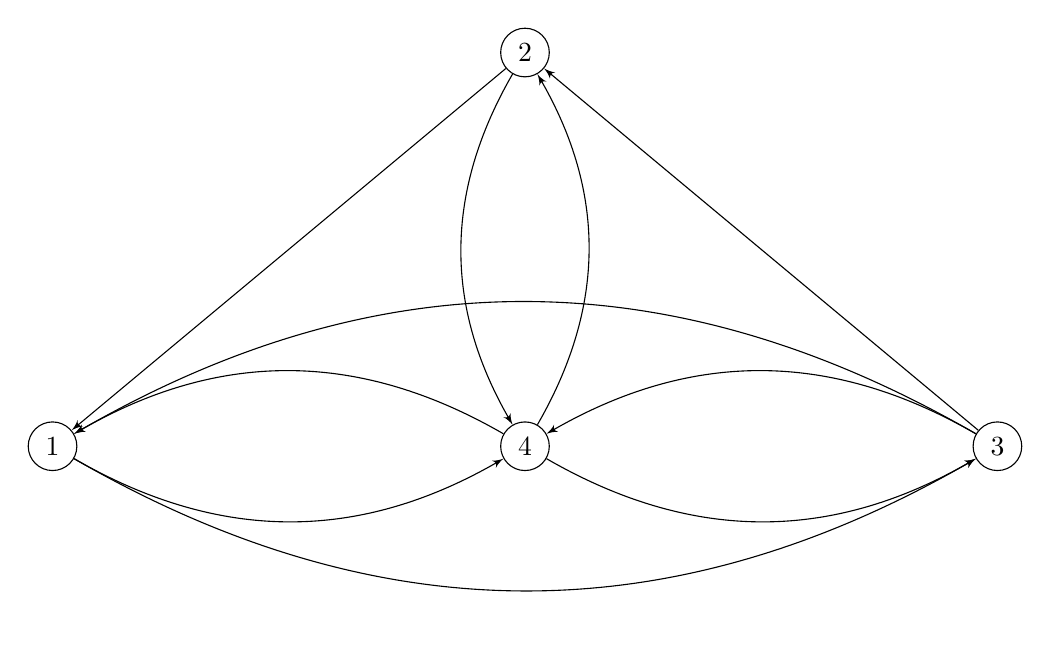
\begin{tikzpicture}

\tikzset{vertex/.style = {shape=circle,draw,minimum size=0.5em}}
\tikzset{edge/.style = {->,> = latex'}}
% vertices
\node[vertex] (1) at  (0,5) {$1$};
\node[vertex] (2) at  (6,10) {$2$};
\node[vertex] (3) at  (12,5) {$3$};
\node[vertex] (4) at  (6,5) {$4$};




%edges

\draw[edge] (1) to[bend right] (3);
\draw[edge] (1) to[bend right] (4);
\draw[edge] (2) to (1);
\draw[edge] (2) to[bend right] (4);
\draw[edge] (3) to (2);
\draw[edge] (3) to[bend right] (1);
\draw[edge] (3) to[bend right] (4); 
\draw[edge] (4)[bend right] to (1); 
\draw[edge] (4)[bend right] to (2); 
\draw[edge] (4)[bend right] to (3); 
\end{tikzpicture}
\end{center}

The following $4\times 4$ matrix is the adjacency matrix of $G$. 
    $$A=\begin{pmatrix}
    0 & 0 & 1 & 1\\
    1 & 0 & 0 & 1\\
    1 & 1 & 0 & 1\\
    1 & 1 & 1 & 0
    \end{pmatrix}.$$ 
We choose another matrix 
    $$A'=\begin{pmatrix}
    0 & 0 & 1 & 1\\
    1 & 0 & 1 & 0\\
    1 & 1 & 0 & 1\\
    1 & 1 & 1 & 0
    \end{pmatrix},$$
which is the adjacency matrix of $G'$ depicted below. 
\bigskip 


\begin{center}
\begin{tikzpicture}

\tikzset{vertex/.style = {shape=circle,draw,minimum size=0.5em}}
\tikzset{edge/.style = {->,> = latex'}}
% vertices
\node[vertex] (1) at  (0,5) {$1$};
\node[vertex] (2) at  (6,10) {$2$};
\node[vertex] (3) at  (12,5) {$3$};
\node[vertex] (4) at  (6,5) {$4$};




%edges

\draw[edge] (1) to[bend right] (3);
\draw[edge] (1) to[bend right] (4);
\draw[edge] (2) to (1);
\draw[edge] (2) to (3);
\draw[edge] (3) to[bend right] (1);
\draw[edge] (3) to (2);
\draw[edge] (3) to[bend right] (4);
\draw[edge] (4)[bend right] to (1);
\draw[edge] (4) to (2);
\draw[edge] (4)[bend right] to (3);
\end{tikzpicture}
\end{center}


Note that both $G$ and $G'$ have the same number of edges, 
neither $A$ majories $A'$ nor $A'$ majories $A$. Our main result still can do comparison between 
$\rho(A)$ and $\rho(A')$. 
We first observe that $A$ is irreducible and $A'$ is $k$-rooted for $k=3$. Moreover 
$A'Q=\begin{pmatrix}
    0 & 0 & 1 & 2\\
    1 & 0 & 1 & 1\\
    1 & 1 & 0 & 1\\
    1 & 1 & 1 & 1
    \end{pmatrix}\geq \begin{pmatrix}
    0 & 0 & 1 & 2\\
    1 & 0 & 0 & 1\\
    1 & 1 & 0 & 1\\
    1 & 1 & 1 & 1
    \end{pmatrix}=AQ$. 
Hence Hence $\rho(A)\leq\rho(A')$ by Theorem~\ref{thm:conclusion} with $C=A$ and $C'=A'$. 
Both of the values of $\rho(C)$ and $\rho(C')$ are close to $2.511547$ by  calculating on computer. \cite[sage]{sage}
\end{exam}

To finish the thesis, we provide an example to show that the `$k$-rooted' assumption of $C'$ is necessary in Theorem~\ref{thm:conclusion}. 

\begin{exam}
    Consider the following two $4\times 4$ matrices
    $$C=\begin{pmatrix}
    0 & 0 & 1 & 1\\
    1 & 0 & 0 & 1\\
    1 & 1 & 0 & 0\\
    1 & 1 & 1 & 0
    \end{pmatrix},\quad C'=\begin{pmatrix}
    0 & 0 & 1 & 1\\
    1 & 0 & 1 &  0\\
    1 & 1 & 0 & 0\\
    1 & 1 & 1 & 0
    \end{pmatrix}.$$
    With $n=4$ and $k=3$, we have  
    $$CQ=\begin{pmatrix}
    0 & 0 & 1 & 2\\
    1 & 0 & 0 & 1\\
    1 & 1 & 0 & 0\\
    1 & 1 & 1 & 1
    \end{pmatrix}\leq \begin{pmatrix}
    0 & 0 & 1 & 2\\
    1 & 0 & 1 & 1\\
    1 & 1 & 0 & 0\\
    1 & 1 & 1 & 1
    \end{pmatrix}=C'Q.$$
Using computer, \cite[sage]{sage}
    $$\rho(C)\approx 2.234\not\leq 2.148\approx \rho(C').$$
    This is because $C'$ is not $k$-rooted as $c'_{33}+c'_{34}=0\not\geq 1=c'_{43}+c'_{44}$.

All theorems come from continuous discussions between C.W. Weng and K.H. Chen. These were all documented.\cite{src_files}
    
\end{exam}


%\section*{References}
\begin{thebibliography}{20}
\normalsize
\addcontentsline{toc}{section}{Bibliography}

\bibitem{chang}
Yen-Jen Cheng, {\it  A matrix realization of spectral bounds
of the spectral radius of a nonnegative matrix}, Ph.D. Thesis, NCTU, 2018.

\bibitem{spec_rad}
A. E. Brouwer, W. H. Haemers, {\it Spectra of graphs}, Springer, 2012
\bibitem{prn_fros2}
R. A. Horn , C. R. Johnson, {\it Matrix analysis}, Cambrigde University Press, 1985.
\bibitem{sage}
[Sage] SageMath, the Sage Mathematics Software System (Version 9.2),
       The Sage Developers, 2020, https://www.sagemath.org.  %sage tutorial
\bibitem{src_files}
[github] K. H. Chen, C. W. Weng, source files to the essay, A simple method on comparison between spectral radii of two directed graphs,
     2021, https://reurl.cc/6yy32Z. % https://github.com/Urbaner3/NCTU_weng. 
    

\end{thebibliography}




\end{document}
